\documentclass[border=10pt]{standalone}
\usepackage[svgnames]{xcolor}
\usepackage{amsmath}
\usepackage{pgfplots}
\pgfplotsset{compat=newest}
\usepackage[sfdefault]{FiraSans}
\usepackage{FiraMono}
\renewcommand*\familydefault{\sfdefault}
\begin{document}
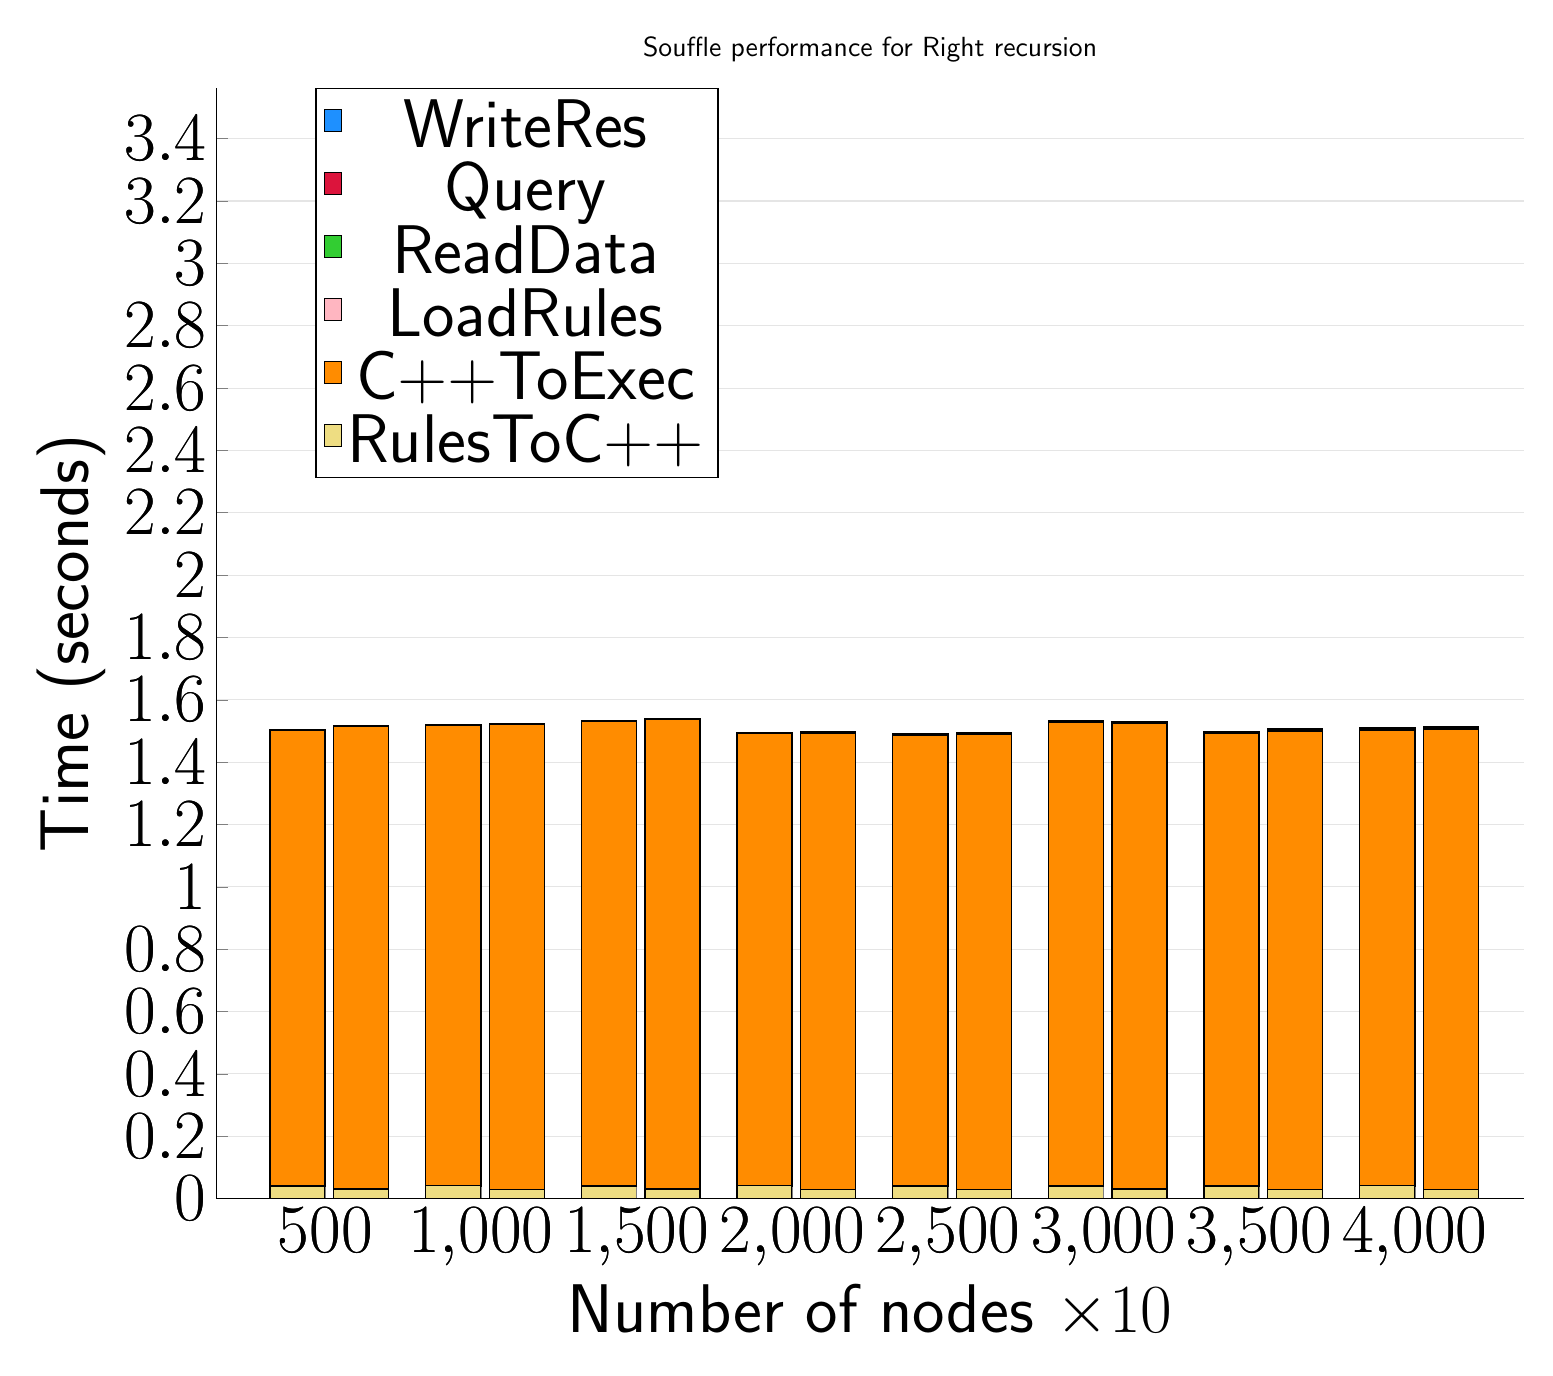
\begin{tikzpicture}
	\begin{axis}[
			ybar stacked,
			title={Souffle performance for Right recursion},
			bar shift=-10pt,
			width=1.5\textwidth,
			bar width=0.7cm,
			ymajorgrids, tick align=inside,
			major grid style={draw=gray!20},
			xtick=data,
			ymin=0, ymax=3.562999987602234,
			axis x line*=bottom,
			axis y line*=left,
			enlarge x limits=0.1,
			legend style={
					at={(0.23, 1)},
					anchor=north,
					legend columns=1,
					font=\Huge,
				},
			ylabel={Time (seconds)},
			xlabel={Number of nodes $\times 10$},
			label style={font=\Huge},
			tick label style={font=\Huge},
		]
		\addlegendimage{fill=DodgerBlue, draw=black, line width=0.2pt}
		\addlegendentry{WriteRes}
		\addlegendimage{fill=Crimson, draw=black, line width=0.2pt}
		\addlegendentry{Query}
		\addlegendimage{fill=LimeGreen, draw=black, line width=0.2pt}
		\addlegendentry{ReadData}
		\addlegendimage{fill=LightPink, draw=black, line width=0.2pt}
		\addlegendentry{LoadRules}
		\addlegendimage{fill=DarkOrange, draw=black, line width=0.2pt}
		\addlegendentry{C++ToExec}
		\addlegendimage{fill=LightGoldenrod, draw=black, line width=0.2pt}
		\addlegendentry{RulesToC++}
		\addplot +[fill=LightGoldenrod, draw=black, line width=0.5pt] coordinates {
				(500, 0.04000000953674317)
				(1000, 0.04100000858306885)
				(1500, 0.039999961853027344)
				(2000, 0.04100000858306885)
				(2500, 0.04000000953674317)
				(3000, 0.039999985694885255)
				(3500, 0.039999961853027344)
				(4000, 0.04100000858306885)
			};
		\addplot +[fill=DarkOrange, draw=black, line width=0.5pt] coordinates {
				(500, 1.4630000114440918)
				(1000, 1.4769999504089355)
				(1500, 1.4910000562667847)
				(2000, 1.450000023841858)
				(2500, 1.4459999799728394)
				(3000, 1.487000012397766)
				(3500, 1.4519999742507934)
				(4000, 1.4619999885559083)
			};
		\addplot +[fill=LightPink, draw=black, line width=0.5pt] coordinates {
				(500, 0.0)
				(1000, 0.0)
				(1500, 0.0)
				(2000, 1.01917e-05)
				(2500, 0.0)
				(3000, 1.00542e-05)
				(3500, 1.06375e-05)
				(4000, 0.0)
			};
		\addplot +[fill=LimeGreen, draw=black, line width=0.5pt] coordinates {
				(500, 0.000421754)
				(1000, 0.0005464874)
				(1500, 0.0006548877000000001)
				(2000, 0.0008252998000000001)
				(2500, 0.0008669374)
				(3000, 0.0009567750999999999)
				(3500, 0.0010582290000000002)
				(4000, 0.001196826)
			};
		\addplot +[fill=Crimson, draw=black, line width=0.5pt] coordinates {
				(500, 0.0006566289999999999)
				(1000, 0.0012235584000000002)
				(1500, 0.0017863640000000004)
				(2000, 0.002493023)
				(2500, 0.0031347470000000002)
				(3000, 0.003521582)
				(3500, 0.0041656969999999995)
				(4000, 0.004851388)
			};
		\addplot +[fill=DodgerBlue, draw=black, line width=0.5pt] coordinates {
				(500, 0.0006072502000000001)
				(1000, 0.00070095)
				(1500, 0.0010360757)
				(2000, 0.0011532920000000002)
				(2500, 0.001364255)
				(3000, 0.0014977299999999999)
				(3500, 0.0017230699999999997)
				(4000, 0.001972853)
			};
	\end{axis}
	\begin{axis}[
			ybar stacked,
			bar shift=13pt,
			width=1.5\textwidth,
			bar width=0.7cm,
			ymajorgrids, tick align=inside,
			major grid style={draw=none},
			xtick=data,
			ymin=0, ymax=3.562999987602234,
			axis x line*=none,
			axis y line*=none,
			enlarge x limits=0.1,
			label style={font=\Huge},
			tick label style={font=\Huge},
		]
		\addplot +[fill=LightGoldenrod, draw=black, line width=0.5pt] coordinates {
				(500, 0.030999999999999993)
				(1000, 0.030000000000000006)
				(1500, 0.030999999999999993)
				(2000, 0.030000000000000006)
				(2500, 0.030000000000000006)
				(3000, 0.030999999999999993)
				(3500, 0.030000000000000006)
				(4000, 0.030000000000000006)
			};
		\addplot +[fill=DarkOrange, draw=black, line width=0.5pt] coordinates {
				(500, 1.485)
				(1000, 1.4900000000000002)
				(1500, 1.5050000000000001)
				(2000, 1.464)
				(2500, 1.459)
				(3000, 1.494)
				(3500, 1.4689999999999999)
				(4000, 1.4750000000000003)
			};
		\addplot +[fill=LightPink, draw=black, line width=0.5pt] coordinates {
				(500, 0.0)
				(1000, 0.0)
				(1500, 0.0)
				(2000, 1.01e-05)
				(2500, 0.0)
				(3000, 1e-05)
				(3500, 1.06e-05)
				(4000, 0.0)
			};
		\addplot +[fill=LimeGreen, draw=black, line width=0.5pt] coordinates {
				(500, 0.0004075)
				(1000, 0.0005214000000000001)
				(1500, 0.000622)
				(2000, 0.000753)
				(2500, 0.0008423999999999999)
				(3000, 0.0009411999999999999)
				(3500, 0.0010289)
				(4000, 0.0011713000000000001)
			};
		\addplot +[fill=Crimson, draw=black, line width=0.5pt] coordinates {
				(500, 0.0006563)
				(1000, 0.0012230000000000003)
				(1500, 0.0017849)
				(2000, 0.0024925000000000004)
				(2500, 0.0031332)
				(3000, 0.0035185999999999993)
				(3500, 0.0041648)
				(4000, 0.0048505)
			};
		\addplot +[fill=DodgerBlue, draw=black, line width=0.5pt] coordinates {
				(500, 0.00044479999999999986)
				(1000, 0.0006732)
				(1500, 0.0009117)
				(2000, 0.0011207)
				(2500, 0.001363)
				(3000, 0.0014960999999999998)
				(3500, 0.0017222000000000001)
				(4000, 0.0019084)
			};
	\end{axis}
\end{tikzpicture}

\end{document}
